\documentclass[italian,10pt,a4paper]{article}
\usepackage[T1]{fontenc}
\usepackage{babel}
\usepackage{graphicx}
\usepackage{subcaption}
\usepackage{hyperref}
\hypersetup{hidelinks}
\usepackage{marvosym}
\hypersetup{
	colorlinks=true,
	linkcolor=black,
	filecolor=magenta,      
	urlcolor=cyan,
	pdfpagemode=FullScreen,
	citecolor=black
}
\graphicspath{{./img/}}

\title{Features extraction dalle immagine di cellule della mucosa nasale}
\author{Vito Proscia\href{v.proscia3@studenti.uniba.it}{\textsuperscript{\Letter}}}
\date{} % clear date

\begin{document}
	\maketitle
	
	\begin{abstract}
		Uno degli step determinanti dell'image analysis, specialmente in ambito biomedico, è l'estrazione delle features da immagini cellulari, la Citologia Nasale è una tecnica clinica utile alla diagnostica in ambito rinoallergologico, essa si basa sull'analisi delle immagini della mucosa nasale, in questo report presentremo tecniche di features extraction per meglio estrarre informazioni da queste immagini cellulari usando varie metodologie quali morphological extraction, texture extraction e color extraction, per poi testare i dati estratti allenando un classificatore con l'obiettivo di meglio catalogare le singole cellule fornendo un supporto al lavoro dei citologi.  
	\end{abstract}
	
	\section{Introduzione}
		
		\subsection{Background}
		
			Le cellule sono l'unità strutturale e funzionale degli organismi viventi, il loro aspetto e la loro morfologia possono rispecchiare la natura biologica dell'organo e persino del corpo, in particolare la citologia nasale è una diagnostica dello studio delle rinopatie, malattie del naso e delle fosse nasali caratterizzato da ostruzione respiratoria, rinorrea (scolo di muco), prurito e starnuti.\\	
			I citologi sono coloro i quali si occupano del processo di estrazione e di analisi delle cellule con l'obiettivo di diagnosticare condizioni infiammatorie e agenti patogeni.\\
			\linebreak
			Con il recente sviluppo delle tecniche di image analysis è stato possibile contribuire al lavoro dei suddetti aiutandoli sia in fase di rilevazione che di classificazione delle singole cellule, la correttezza di questi modelli è in larga parte determinata dal processo di features extraction che, in questo caso, consiste nel carpire le informazioni rilevanti dalle immagini delle cellule.
			
			\subsection{Cellule della mucosa nasale}
			
				\subsubsection{Estrazione}
					Inizialmente si dilata la narice con uno \textit{Speculum} nasale, successivamente si preleva con il Rhinoprobe una quantità di materiale cellulare dalla mucosa nasale, infine si striscia il materiale su un vetrino e lo si colora, essendo trasparente, con \textit{May Grumwald Giemsa}, un colorante tendente al viola.
					
			
				\subsubsection{Tipologie di cellule}
					In una mucosa nasale si possono trovare, nelle giuste proporzioni, diverse popolazioni di cellule, tra quelle che compongono il dataset fornito possiamo distinguere:
					
					\begin{itemize}
						\item \textit{Ciliate}: cellule epiteliali più comuni, responsabili del movimento del muco, sono caratterizzate dal nucleo situato ad un’altezza variabile dal fondo della cellula e dalle “ciglia” situate in alto;
						
						\item \textit{Mucipare}: responsabili della produzione di muco, l’insieme di queste cellule ha la funzione di creare un flusso costante di fluido che si scarica nella faringe;
						
						\item \textit{Neutrofili}: caratterizzate da più nuclei legati da sottilissimi filamenti di materiale nucleare all'interno del citoplasma;
						
						\item \textit{Mastociti}: cellule immunitarie rotondeggianti od ovali composti da granuli circondati da membrana, intervengono nella genesi delle reazioni allergiche, di ipersensibilità e anafilattiche;
						
						\item \textit{Linfociti}: analizzano i germi che penetrano attraverso il naso memorizzandoli per poi preparare la produzione di anticorpi specifici, caratterizzate dall’avere un nucleo molto grande che ricopre quasi interamente la superficie della cellula stessa;
						
						\item \textit{Granulociti eobsinofili}: tipo di globuli bianchi che hanno funzione di difesa dell'organismo, caratterizzati dall’avere due nuclei collegati tra loro;
						
						\item \textit{Metaplastiche}: espressione di infiammazione cronica;
		
						\item \textit{Batteri}: indice di un'infiammazione batterica in corso.
						
					\end{itemize} 
			
					\begin{figure}[h]
						\centering
						\begin{subfigure}[h]{70px}
							\centering
							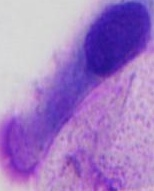
\includegraphics[width=2cm, height=2cm]{ciliate.jpg}
							\caption{Ciliate}
							\label{fig:image1}
						\end{subfigure}
						\hfill
						\begin{subfigure}[h]{70px}
							\centering
							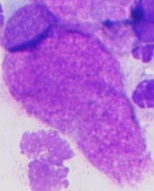
\includegraphics[width=2cm, height=2cm]{mucipare.jpg}
							\caption{Mucipare}
							\label{fig:image2}
						\end{subfigure}
						\hfill
						\begin{subfigure}[h]{70px}
							\centering
							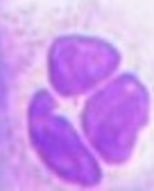
\includegraphics[width=2cm, height=2cm]{neutrofili.jpg}
							\caption{Neutrofili}
							\label{fig:image3}
						\end{subfigure}
		
						\label{fig:multiple_images1}
						\begin{subfigure}[h]{70px}
							\centering
							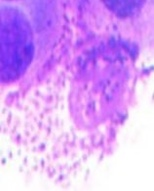
\includegraphics[width=2cm, height=2cm]{mast.jpg}
							\caption{Mastociti}
							\label{fig:image4}
						\end{subfigure}
						\hfill
						\begin{subfigure}[h]{70px}
							\centering
							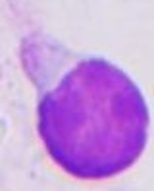
\includegraphics[width=2cm, height=2cm]{linfociti.jpg}
							\caption{Linfociti}
							\label{fig:image5}
						\end{subfigure}
						\hfill
						\begin{subfigure}[h]{70px}
							\centering
							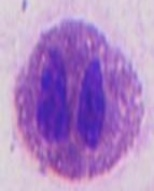
\includegraphics[width=2cm, height=2cm]{eosinophil.jpg}
							\caption{Granulociti}
							\label{fig:image6}
						\end{subfigure}
		
						\label{fig:multiple_images2}
						\begin{subfigure}[h]{70px}
							\centering
							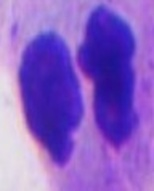
\includegraphics[width=2cm, height=2cm]{metaplatic.jpg}
							\caption{Metaplastiche}
							\label{fig:image7}
						\end{subfigure}
						\hfill
						\begin{subfigure}[h]{70px}
							\centering
							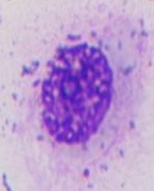
\includegraphics[width=2cm, height=2cm]{epiteliali.jpg}
							\caption{Epiteliali}
							\label{fig:image8}
						\end{subfigure}
						\hfill
						\begin{subfigure}[h]{70px}
							\centering
							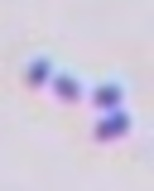
\includegraphics[width=2cm, height=2cm]{batteri.jpg}
							\caption{Batteri}
							\label{fig:image9}
						\end{subfigure}
						
						\caption{Differenti tipologie di cellule nel dataset}
						\label{fig:multiple_images3}
					\end{figure}
		
	\section{Materiali e metodi}
		In questa sezione approfondiremo come si è andati ad elaborare il dataset ed i successivi metodi di features extraction, per poi effettuare un test delle features ottenute andando ad allenare, su queste, un classificatore con l'obiettivo di discriminare il tipo delle cellule. \footnote{Link sperimentazione: \href{https://github.com/Giut0/Nasal-Cell-Feature-Extraction}{https://github.com/Giut0/Nasal-Cell-Feature-Extraction}}
		
		\subsection{Image processing}
			Originariamente il dataset ricevuto era composto da una serie di immagini di cellule, ogni immagine contava più cellule insieme, tutte annotate con le rispettive coordinate e classi di appartenenza.\\
			Per i nostri scopi si è andati ad isolare ogni singola cellula dalle immagini originali, per poi prodourre un file che contenesse i nomi delle immagini delle singole cellule e le loro classi corrispondenti.
			
		\subsection{Features extraction}
			Per caratterizzare ogni singola cellula isolata è necessario estrarre, da queste, delle informazioni, per poi usare il tutto allenando un classificatore.\\
			In questo caso si è pensato di combinare tre differenti tipologie di features:
			
				\subsubsection{Feature morfologiche}
					Le caratteristiche morfologiche includono dimensioni, forme e bordi delle cellule, si sono ottenute convertendo ogni immagine in bianco e nero, successivamente trovando i contorni (massimo 2 in questo caso essendo cellule isolate quindi cellula stessa e nucleo) ed infine per ogni contorno trovato si salvano sia l’area che il perimetro.
					
				\subsubsection{Feature di texture}
					Le caratteristiche della texture descrivono le variazioni nei livelli di grigio all'interno dell'immagine, per questo scopo si sono usate le matrici di co-occorrenza a livello di grigio (GLCM) \cite{liu_feature_2013}, strumento per l’analisi delle texture di un’immagine in scala di grigi, misura la frequenza di coppie di pixel con valori d’intensità specifici (livelli di grigio) ad una data distanza e angolo (nel nostro caso specifico la distanza di valutazione è stata impostata a 1 e l'angolo a 0°), le informazioni ottenibili con questo strumento sono :
					
					\begin{itemize}
						
						\item \textbf{Contrasto}: indica quanto variano i livelli di grigio tra i pixel vicini; $$\sum_{i,j=0}^{levels-1} P_{i,j}(i-j)^2$$
						
						\item \textbf{Dissimilarità}: simile al contrasto, ma tiene conto solo della differenza assoluta tra i livelli di grigio dei pixel vicini, senza elevarla al quadrato; $$\sum_{i,j=0}^{levels-1}P_{i,j}|i-j|$$
						
						\item \textbf{Omogeneità}: misura quanto i pixel vicini sono simili in termini di intensità; $$\sum_{i,j=0}^{levels-1}\frac{P_{i,j}}{1+(i-j)^2}$$
						
						\item \textbf{Energia}: misura la quantità di ordine e ripetitività nella texture, valori elevati di energia indicano una texture altamente strutturata e ripetitiva; $$\sqrt{\sum_{i,j=0}^{levels-1} P_{i,j}^2}$$
						
						\item \textbf{Correlazione}: misura quanto una coppia di pixel varia in modo correlato rispetto alla media. $$\sum_{i,j=0}^{levels-1} P_{i,j}\left[\frac{(i-\mu_i) \
							(j-\mu_j)}{\sqrt{(\sigma_i^2)(\sigma_j^2)}}\right]$$
						
					\end{itemize}
					
				\subsection{Feature di colore}
					Le caratteristiche del colore sono importanti per descrivere le proprietà visive delle immagini delle cellule, in questo, caso per ogni immagine, si è andati a salvare l'istogramma dei colori \cite{Baker_2021}.
				 			
		\subsection{Classificazione}
		
			Le features estratte sono state successivamente testate allenando il modello \textbf{Random Forest}, modello \textit{ensambled} di apprendimento automatico supervisionato che combina molteplici alberi decisionali, ognuno dei quali addestrato su un subset casuale dei dati, per migliorare le previsioni.\\ 
			\linebreak
			Dopo varie sperimentazioni si riporta la migliore configurazione del modello:
			
			\begin{enumerate}
				
				\item \texttt{n\_estimators = 200}, rappresenta il numero di alberi su cui lavorare;
				\item  \texttt{criterion = "gini"}, criterio di \textit{split} degli alberi, in particolare il criterio punta a minimizzare l'impurità dei nodi, quindi per scegliere l'attributo che meglio divide i dati in base alla target feature per ogni nodo si calcola:
				$$GINI(v) = 1-\sum_{i = 1}^{|C|}p_i^2$$
				dove:
				\begin{itemize}
					\item $v$ è il nodo in esame;
					\item $C$ rappresenta l'inseme delle classi;
					\item $p_i$ è la probabilità che un campione nel nodo $v$ appartenga alla classe $i$.
				\end{itemize}
				infine vene scelto il nodo con minor impurità. \\
				\linebreak
				L'indice \texttt{gini} è stato scelto per la sua efficenza, infatti la complessità per il calcolo dell'indice per uno nodo è dell'ordine di $O(c)$, dove c è il numero di classi.
				
		\end{enumerate}

	\section{Risultati}
		Per andare a valutare il modello ottenuto si sono scelte le metriche più comuni:
		
		\begin{table}[h]
			\centering
			\begin{tabular}{|l|c|}
				\hline
				\textbf{Metrica} & \textbf{Valore} \\
				\hline
				Accuracy & 0.800 \\
				\hline
				Precision & 0.782 \\
				\hline
				Recall & 0.800 \\
				\hline
			\end{tabular}
			\caption{Risultati della classificazione}
		\end{table}
		
	\section{Conslusioni}
	L'obiettivo principale della sperimentazione è l'estrazione di features da immagini cellulari della mucosa nasale, in primo luogo siamo andati ad isolare le singole cellule dalle immaigni utilizzando le coordinate fornite, successivamente c'è stata la fase di feature extraction andando a combinare tre differenti metodologie quali morphological extraction, texture extraction e color extraction ed infine abbiamo provato ad allenare un classificatore sui dati ottenuti raggiungendo dei buoni risultati.\\
	Tuttavia, ci sono ancora ampi margini di miglioramento che possono aiutare il modello ad effettuare delle migliori predizioni, magari provando a combinare il tutto con altre tecniche come la trasformata di Fourier, oppure intraprendendo la strada del deep learning.
	
	
	\bibliographystyle{unsrt}
	\bibliography{stsmult}
	

\end{document}